\section{Extensions}\label{sec:extension}

WAIT and Nested WAIT extend naturally in two directions: time-varying arrivals $\lambda_j^t$ (using accumulated arrival constraints) and segment-wise design (grouping $m$ types into $L \leq m$ segments). Both extensions preserve asymptotic optimality.

\subsection{Time-Varying Arrival Rates}\label{sec:time_varying}

For time-varying $\lambda_j^t$, replace constant rates with accumulated arrivals $\lambda_j[t_1, t_2] := \int_{t_1}^{t_2} \lambda_j^t \, dt$. Threshold conditions \eqref{eq:nested_wait_thresholds} generalize to: for all $t\in [0, T]$, $0<\Delta t\leq \Delta T$, and $k = 1, \dots, m-1$,
\begin{equation}
    \label{eq:nested_wait_thresholds_time_varying}
    \sum_{j=1}^m \lambda_j[t, t + \Delta t] < n_1, \quad n_{k+1}/n_k > p_k[t,t+\Delta t],
\end{equation}
where $p_k[t,t+\Delta t] = (\sum_{j=k+1}^m\lambda_j[t,t+\Delta t])/(\sum_{j=k}^m\lambda_j[t,t+\Delta t])$.

\begin{theorem}
\label{thm:nested_wait_heavy_traffic_time_varying}
Under these time-varying thresholds with safety buffer $M^{(\zeta,\pi)} = O( 2M^\pi + \sum_{k=1}^m \theta_k^{-1}  (l + l_{k-1}') \ln( m \zeta B/\delta ))$, Nested WAIT achieves $\throughput^* - \mathbb{E}[ \throughput^{(\zeta, \pi)}] = O((\zeta T)^{-1})$, $\mathbb{E}[\Latency^{(\zeta, \pi)}] = O(1)$, with overflow probability $< \delta$.
\end{theorem}

The coupling construction extends naturally using time-varying Poisson processes. Proof in Appendix~\ref{appendix:: proof of nested optimality, time varying.}.

\subsection{Segment Design}\label{sec:segment_design}

The \textbf{segment-wise design} groups $m$ types into $L \leq m$ segments (e.g., $L=10$ for $m=500$ in LMSYS~\cite{zheng2023lmsys}), reducing complexity from $O(m)$ to $O(L)$. Partition types with decode lengths $l_1' < \cdots < l_m'$ into $L$ segments with $\Delta L:= m/L$ types each. Segment $k$ has aggregate rate $\lambda_k' = \sum_{(k-1)\Delta L+1\le j\le k\Delta L} \lambda_j$.

Given a policy $\pi=[n_1,\dots,n_L]$ with threshold $n_k$ for the $k$-th segment in Algorithm \ref{alg:nested_wait}, we formulate a linear system analogous to Equation \eqref{eq:nested_wait_thresholds}:
\begin{equation}          \label{eq:nested_wait_thresholds_L}
    \begin{aligned}
    &\Delta T_{[1:L]}(n_{1:L}) \leq \frac{n_1}{\sum_{r=1}^L \lambda_r'},  \\
    &\frac{n_{k+1}}{n_k} > p_k, \ \forall k < L,
    \end{aligned}
\end{equation}
where $p_k =\frac{\lambda'(k+1 \to L)}{\lambda'(k \to L)}$, $\Delta T_{[1,\dots,L]}(n_1,\dots,n_L) = d_0 + d_1 M^\pi(n_1, \dots, n_L)$, and memory is:
\[
M^{\pi}(n_1, \dots, n_L) = \sum_{k=1}^L n_k \left( l + \frac{k}{2} \Delta L\right) \Delta L.
\]

\begin{theorem}
\label{thm:nested_wait_heavy_traffic, any segment}
If $\pi = [n_1, \dots, n_L]$ satisfies \eqref{eq:nested_wait_thresholds_L} and $M^{(\zeta, \pi)} = O( 2M^\pi + \sum_{k=1}^L (l + l_{k-1}') \theta_k^{-1} \ln(m \zeta B/\delta))$, then $\throughput^* - \mathbb{E}[\throughput^{(\zeta, \pi)}] = O((\zeta T)^{-1})$, $\mathbb{E}[\Latency^{(\zeta, \pi)}] = O(1)$, $\mathbb{E}[\TTFT^{(\zeta, \pi)}] = O(1)$, with overflow probability $< \delta$ over $[0, T]$.
\end{theorem}

Proof follows Theorem~\ref{thm:nested_wait_heavy_traffic} in Appendix~\ref{appendix::proof of nested_wait_heavy_traffic}: aggregated rates preserve the Poisson coupling structure.

Figure~\ref{fig:fixed_T_200_rate_500_delta_0.1_1e-5} validates using LMSYS data ($m = 500$): total memory exhibits U-shape with minimum at $L=5$-$10$, confirming $L=10$ (Section~\ref{sec:experiments}).

\begin{figure}[ht]
    \centering
    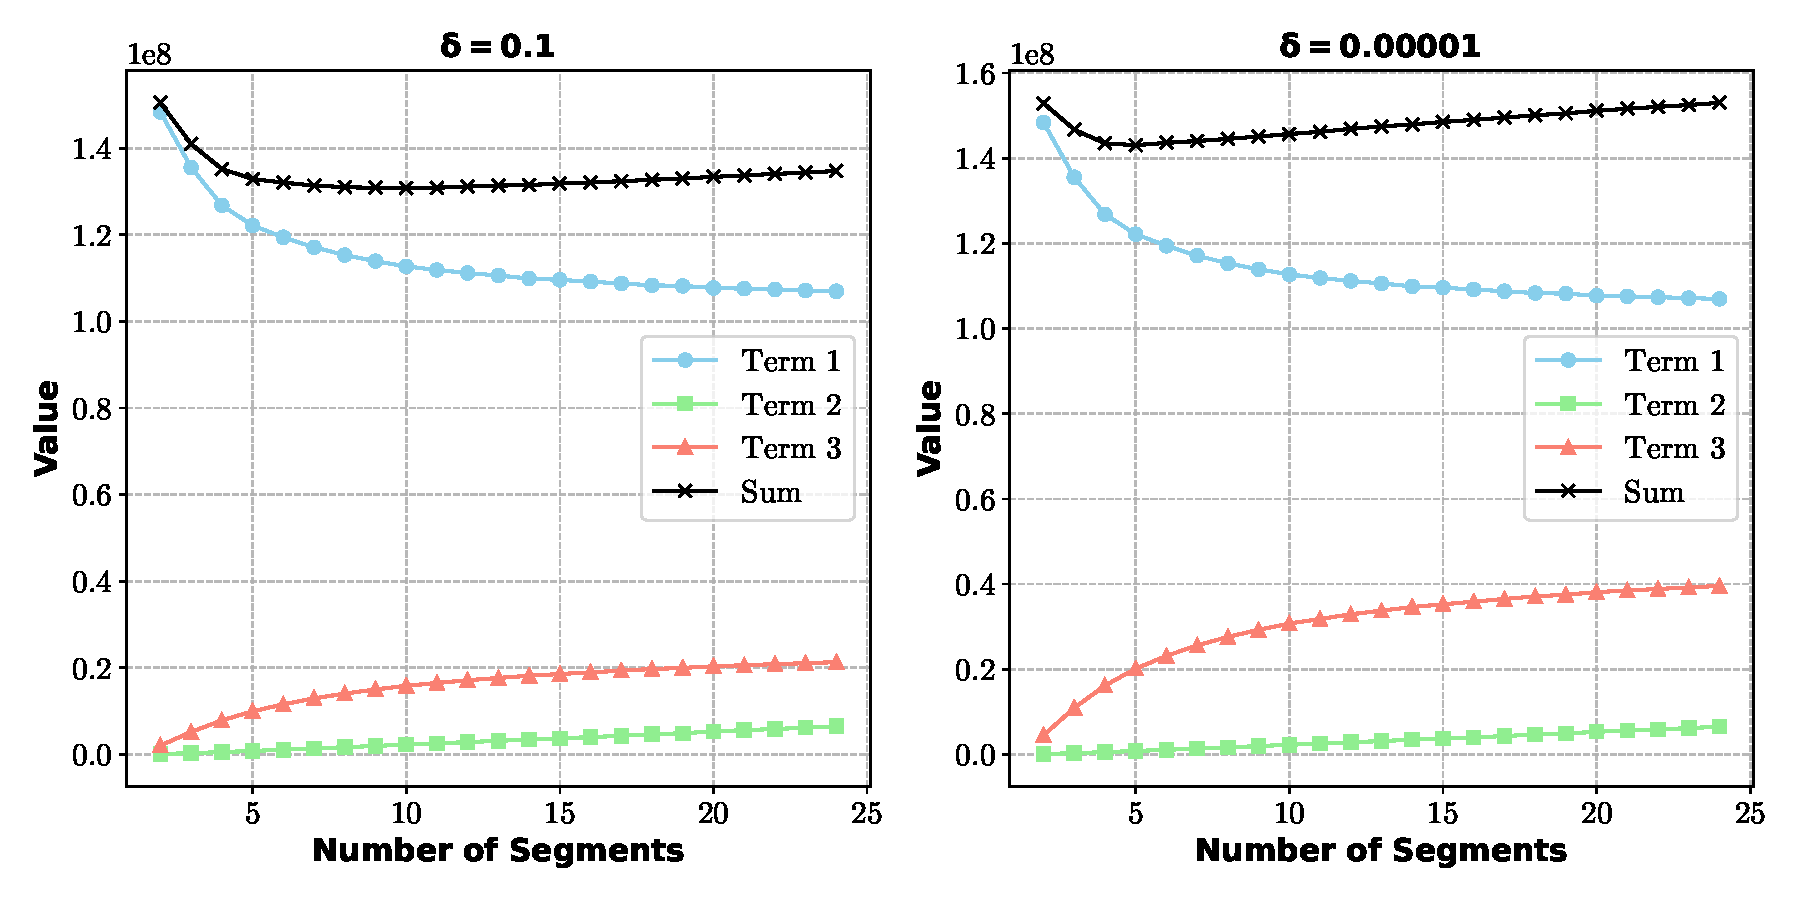
\includegraphics[width=0.6\textwidth]{Experiments_pdf/total_rate=500,T=200.pdf}
    \caption{Memory components vs. segments $L$ (rate=500, $T=200$). Left: $\delta=0.1$; Right: $\delta=10^{-5}$.}
    \label{fig:fixed_T_200_rate_500_delta_0.1_1e-5}
\end{figure}

% \subsection{Different prefill length}
% For the analysis of Nested WAIT, we assume that the prefill lengths of different prompts are all $l$.



% \subsection{Optimality under arbitrary segments}
% \gan{Maybe this subsection should be put later.}

